\documentclass[11pt, oneside]{article}   	% use "amsart" instead of "article" for AMSLaTeX format
\usepackage{geometry}                		% See geometry.pdf to learn the layout options. There are lots.
\geometry{letterpaper}                   		% ... or a4paper or a5paper or ... 
%\geometry{landscape}                		% Activate for for rotated page geometry
%\usepackage[parfill]{parskip}    		% Activate to begin paragraphs with an empty line rather than an indent
\usepackage{graphicx}				% Use pdf, png, jpg, or eps� with pdflatex; use eps in DVI mode
								% TeX will automatically convert eps --> pdf in pdflatex		
\usepackage{amssymb}
\usepackage{amsmath}
\usepackage{parskip}

\title{Two Determinant Proofs}
%\author{The Author}
%\section{}
% \subsection*{R code}
\date{}							% Activate to display a given date or no date

\graphicspath{{/Users/telliott_admin/Dropbox/Tex/png/}}

% \begin{center} 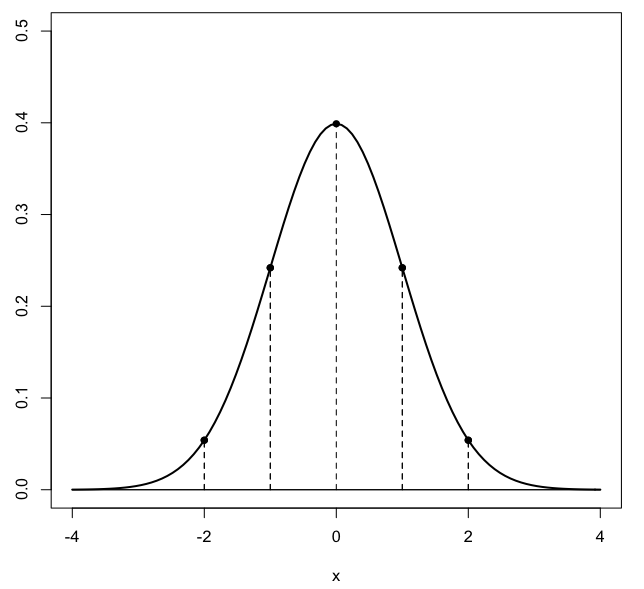
\includegraphics [scale=0.4] {gauss3.png} \end{center}
% \begin{bmatrix} a  &  b \\ c  &  d \end{bmatrix}
% \bigg |_

\begin{document}
\maketitle
\Large
%\noindent
In this short write-up we will prove two basic identities for determinants:
\[ |\mathbf{AB}| = |\mathbf{A}|\ |\mathbf{B}| \]
\[ |\mathbf{A}| = |\mathbf{A}^T| \]

\subsection*{$|\mathbf{AB}| = |\mathbf{A}|\ |\mathbf{B}|$}

Strang does something interesting here (proving the $n \times n$ case by algebra is complicated).  If $\mathbf{B}$ is zero, this equation is certainly true.

If $\mathbf{B}$ is non-zero then consider this ratio:
\[ D(A) = \frac{|\mathbf{AB}|}{|\mathbf{B}|} \]  

Does $D(A)$ have the first three properties that define the determinant of $A$?  If $A=I$ then this becomes

\[ D(A) = \frac{|\mathbf{B}|}{|\mathbf{B}|} = 1 \]  For property 2, if two rows of $A$ are exchanged, then so are the same two rows of $AB$ and therefore $|AB|$ changes sign, and so does the ratio $D(A)$.

Finally property 3 (linearity) also holds (check for yourself).

Since the ratio $D(A)$ has the same three properties that define $|A|$, it equals $|A|$.

Note that if this is given then:

\[ A A^{-1} = I \]
\[
\begin{vmatrix}
A
\end{vmatrix}
\begin{vmatrix}
A^{-1}
\end{vmatrix}
=
\begin{vmatrix}
I
\end{vmatrix}
= 1
\]
\[ |A| = \frac{1}{|A^{-1}|} \]

\subsection*{$|\mathbf{A}| = |\mathbf{A}^T|$}

The simplest way to see this is use the rules for computing determinants of e.g. $3 \times 3$

\[
\begin{vmatrix}
a & b & c \\
d & e & f \\
g & h & i
\end{vmatrix}
=
a(ei - hf) - b(di - fg) + c(dh - eg) \]

Now, the transpose is

\[ 
\begin{vmatrix}
a & d & g \\
b & e & h \\
c & f & i
\end{vmatrix}
=
a(ei - hf) - d(bi - ch) + g(bf - ec) \]

All the same terms are there.  But we haven't proved these rules yet

To Prove:  $|\mathbf{A}| = |\mathbf{A}^T|$

Either $\mathbf{A}$ is \emph{singular} with determinant zero (and so is its transpose), or it can be factored into triangular matrices $\mathbf{L}$ and $\mathbf{U}$.


To do this, the rows of $\mathbf{A}$ may need to be reordered first by multiplication with a permutation matrix $\mathbf{P}$.  Thus
\[ \mathbf{P} \mathbf{A} = \mathbf{L} \mathbf{U} \]

Let's start with the permutation matrix.  $\mathbf{P}$ has determinant either $\pm 1$, by rule 2  (from the previous write-up).  

For any permutation matrix, the transpose is also the inverse
\[ \mathbf{P}^T = \mathbf{P}^{-1} \]
so
\[ \mathbf{P} \mathbf{P}^T = \mathbf{I} \]

(since any row or column of either has at most a single $1$, and those match up in the row by column multiplication because of the transpose.

We proved above that
\[ |\mathbf{AB}| = |\mathbf{A}|\ |\mathbf{B}|  \]
Let's call this the product rule.  By using this rule and then that the determinant of the identity matrix is $1$
\[ 
\begin{vmatrix} \mathbf{P} \end{vmatrix}
\begin{vmatrix} \mathbf{P}^T \end{vmatrix}
=
\begin{vmatrix} \mathbf{P}\mathbf{P}^T \end{vmatrix}
=
\begin{vmatrix} \mathbf{I} \end{vmatrix}
= 1
\]

Now, either $\begin{vmatrix} \mathbf{P} \end{vmatrix} = 1$ and so, by the last equation, $\begin{vmatrix} \mathbf{P}^T \end{vmatrix} = 1$, or else both determinants are minus 1.  

In either case
\[ \begin{vmatrix} \mathbf{P} \end{vmatrix} = 
\begin{vmatrix} \mathbf{P}^T \end{vmatrix}
\]

Moving to the right-hand side
\[
\begin{vmatrix} \mathbf{U} \end{vmatrix}
= 
\begin{vmatrix} p  &  a & b \\ 0  &  q & c \\ 0 & 0  &  r \end{vmatrix}
\]

By rule 7 (previous write-up), $|\mathbf{U}| = pqr$.  Transposition doesn't change the values on the diagonal, so the determinant of a triangular matrix is not changed by the transpose.
\[
\begin{vmatrix} \mathbf{U} \end{vmatrix}
=
\begin{vmatrix} \mathbf{U}^T \end{vmatrix}
\]

There is a particular decomposition into $\mathbf{LU}$ in which $\mathbf{L}$ has $1$'s on the diagonal, although that's not required for what comes next.  But in that case, $|\mathbf{L} | = 1$.  Otherwise

\[
\begin{vmatrix} \mathbf{L} \end{vmatrix} 
=
\begin{vmatrix} u  &  0 & 0 \\ x  &  v & 0 \\ y & z  &  w \end{vmatrix}
= 1
\]
and so (again, since transposition doesn't change the diagonal entries), $|L| = |L^T|$.

\section*{putting it all together}
We have that
\[ \mathbf{PA} =  \mathbf{LU} \]
and we have shown that individually, each of $\mathbf{P}$, $\mathbf{L}$ and $\mathbf{U}$ has the same determinant as the respective transpose.  Further, we have the product rule, $|\mathbf{AB}| = |\mathbf{A}| |\mathbf{B}|$.

Now since
\[ \mathbf{PA} =  \mathbf{LU} \]
\[ |\mathbf{PA}| =  |\mathbf{LU}| \]
and
\[ (\mathbf{PA})^T =  (\mathbf{LU})^T \]
\[ |(\mathbf{PA})^T| =  |(\mathbf{LU})^T| \]

Looking first at the right hand side, by the property of the transpose
\[ |(\mathbf{LU})^T| = |\mathbf{U}^T \mathbf{L}^T| \]
by the product rule
\[ |\mathbf{U}^T \mathbf{L}^T| =  |\mathbf{U}^T| |\mathbf{L}^T|\]
by the identities above
\[ = |\mathbf{U}| |\mathbf{L}|\]
\[ = |\mathbf{L}| |\mathbf{U}|\]
by the product rule
\[ = |\mathbf{LU}|\]

In summary
\[ |(\mathbf{PA})^T|= |\mathbf{LU}|\]

by our initial formulation
\[ |\mathbf{PA}| = |\mathbf{LU}| \]


Thus, we have shown that 
\[ |\mathbf{PA}| = |(\mathbf{PA})^T| \]
but by the product rule
\[ |\mathbf{PA}| = |\mathbf{P}| |\mathbf{A}| \]
and by the property of the transpose
\[ (\mathbf{PA})^T = \mathbf{A}^T \mathbf{P}^T \]
so
\[ |(\mathbf{PA})^T| = | \mathbf{A}^T \mathbf{P}^T  |\]
by the product rule 
\[ = | \mathbf{A}^T | | \mathbf{P}^T  |\]
Thus
\[ |\mathbf{PA}| = |(\mathbf{PA})^T| \]
\[ |\mathbf{P}| |\mathbf{A}| = | \mathbf{A}^T | | \mathbf{P}^T  |\]
but 
\[ |\mathbf{P}| = | \mathbf{P}^T  |\]
so
\[ |\mathbf{A}| = | \mathbf{A}^T  |\]

\end{document}  